\chapter{Oksidasi dan Reduksi}\label{ch:g11:redox}

Sekeping seng dicelupkan ke dalam larutan tembaga sulfat yang biru.
Dalam beberapa menit permukaannya menjadi gelap tertutup lapisan cokelat
kemerahan yang seperti spons; sejam kemudian warna biru larutan itu
telah memudar. \omterm{def:g9:periodic-table-first-look:metal}{Logam} tembaga muncul di tempat yang tadinya tidak ada,
dan seng telah masuk ke dalam larutan sebagai \omterm{def:g9:ions:ion}{ion} yang tidak terlihat.
Tidak ada yang dipanaskan, tidak ada gas yang dilepaskan, tidak ada
oksigen yang ikut serta --- namun para ahli kimia menyebut peristiwa ini
\omterm{def:g11:redox:oxidation}{oksidasi}. Kata itu dulu berarti ``bergabung dengan oksigen''; kini
artinya lebih umum dan lebih berguna: pelepasan \omterm{def:g9:inside-the-atom:nucleus}{elektron}. Bab ini
mengikuti jejak \omterm{def:g9:inside-the-atom:nucleus}{elektron-elektron} itu.

\begin{recall}
\omterm{def:g9:ions:ion}{Ion} adalah \omterm{def:g7:atoms-and-molecules:atom}{atom} atau sekelompok \omterm{def:g7:atoms-and-molecules:atom}{atom} yang telah menerima atau melepaskan
\omterm{def:g9:inside-the-atom:nucleus}{elektron} (\cref{ch:g9:ions}). \omterm{def:g9:periodic-table-first-look:metal}{Logam} seperti besi atau seng bereaksi
dengan asam klorida menghasilkan hidrogen dan \omterm{def:g9:ions:ion}{ion} \omterm{def:g9:periodic-table-first-look:metal}{logam}
(\cref{ch:g9:metals-acids-corrosion}). \omterm{def:g10:the-mole:amount}{Jumlah zat} $n$, dalam \omterm{def:g10:the-mole:amount}{mol},
dihitung dari massa $m$ dengan $n = m/M$ (\cref{ch:g10:the-mole}).
\end{recall}

\begin{omfigure}
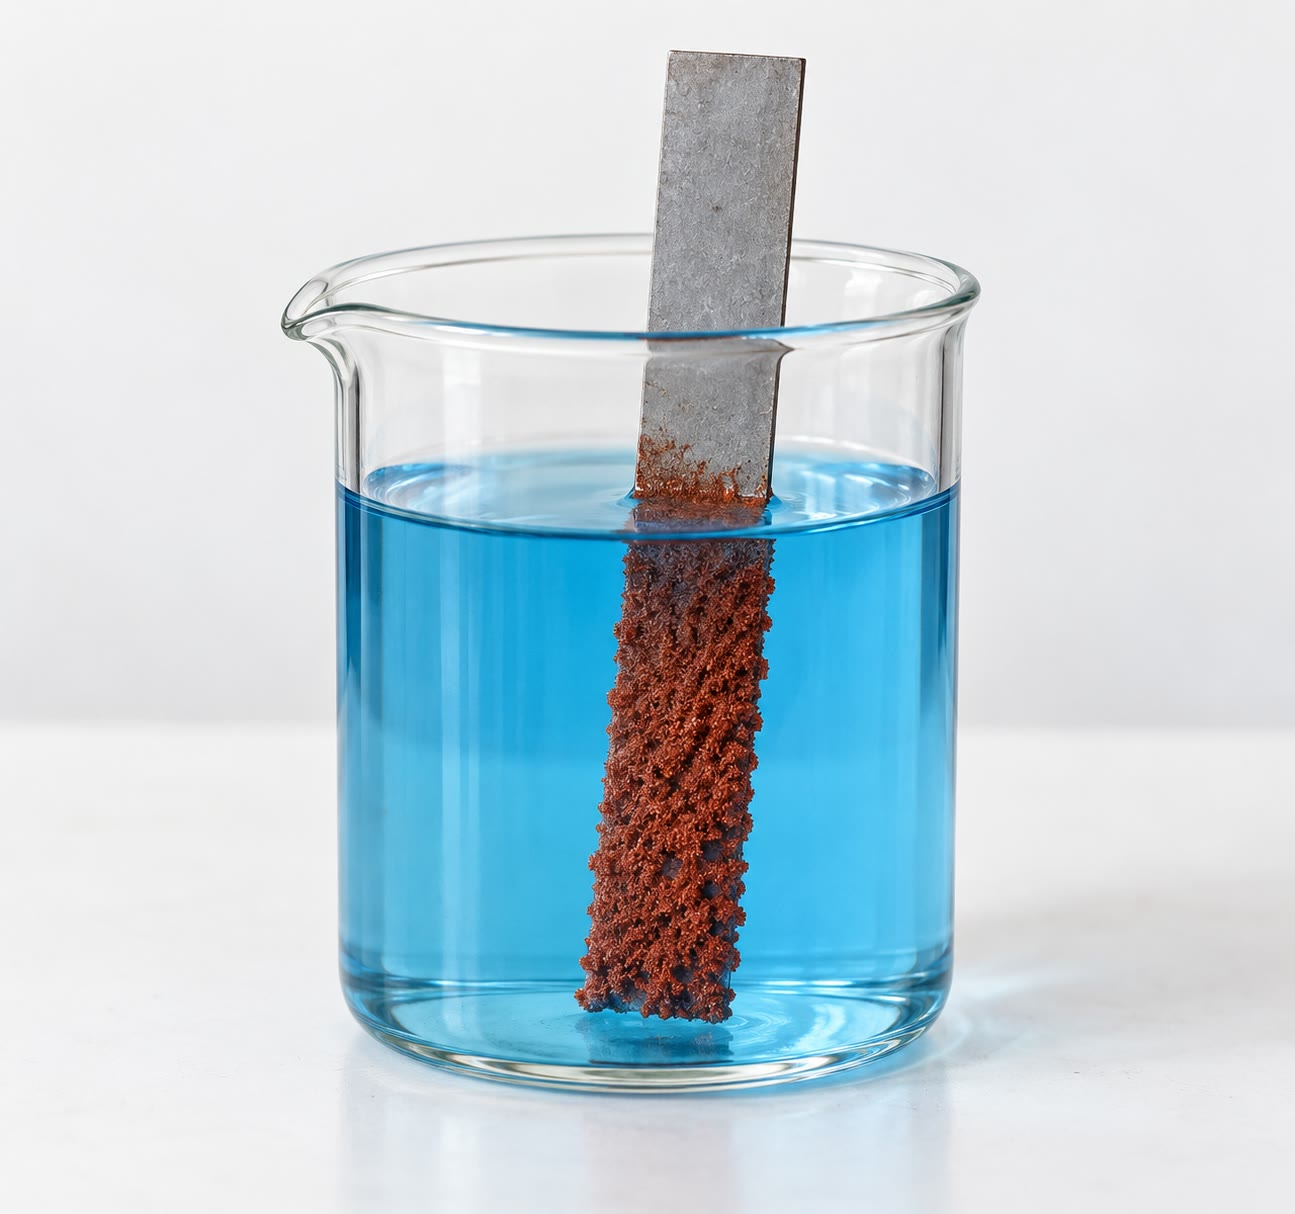
\includegraphics[width=0.55\linewidth]{images/book1/ai/g11-zinc-copper-sulfate.jpg}

{\small Sekeping seng dalam larutan tembaga sulfat: tembaga mengendap pada
seng, dan \omterm{def:g9:ions:ion}{ion-ion} seng menggantikan tempatnya di dalam larutan.}
\end{omfigure}

\section{Oksidator dan reduktor}

\begin{definition}[Oksidator dan reduktor]\label{def:g11:redox:oxidant}
Sebuah \emph{oksidator}\index{oksidator} adalah spesies yang mampu
menerima satu \omterm{def:g9:inside-the-atom:nucleus}{elektron} atau lebih. Sebuah \emph{reduktor}\index{reduktor}
adalah spesies yang mampu memberikan satu \omterm{def:g9:inside-the-atom:nucleus}{elektron} atau lebih.
\end{definition}

\begin{definition}[Oksidasi dan reduksi]\label{def:g11:redox:oxidation}
Yang disebut \emph{oksidasi}\index{oksidasi} adalah pelepasan \omterm{def:g9:inside-the-atom:nucleus}{elektron};
yang disebut \emph{reduksi}\index{reduksi} adalah penerimaan \omterm{def:g9:inside-the-atom:nucleus}{elektron}.
\omterm{def:g11:redox:oxidant}{Reduktor} dioksidasi; \omterm{def:g11:redox:oxidant}{oksidator} direduksi.
\end{definition}

\begin{remark}[Cara mengingatnya]\label{rem:g11:redox:remember}
Pada \emph{\omterm{def:g11:redox:oxidation}{reduksi}}, muatan spesies itu berkurang: \ce{Cu^{2+}} yang
menerima dua \omterm{def:g9:inside-the-atom:nucleus}{elektron} menjadi \ce{Cu}, muatan $+2 \to 0$. Pada \omterm{def:g11:redox:oxidation}{oksidasi}
muatannya naik: \ce{Zn -> Zn^{2+} + 2e-}, $0 \to +2$.
\end{remark}

\begin{definition}[Pasangan redoks dan setengah reaksi]\label{def:g11:redox:couple}
Sebuah \omterm{def:g11:redox:oxidant}{oksidator} dan \omterm{def:g11:redox:oxidant}{reduktor} yang terbentuk darinya dengan menerima
\omterm{def:g9:inside-the-atom:nucleus}{elektron} membentuk sebuah \emph{pasangan redoks}\index{pasangan redoks},
yang ditulis Oks/Red dengan \omterm{def:g11:redox:oxidant}{oksidator} di depan: \ce{Cu^{2+}}/\ce{Cu},
\ce{Zn^{2+}}/\ce{Zn}. Pertukaran \omterm{def:g9:inside-the-atom:nucleus}{elektron} di dalam sebuah pasangan
dinyatakan dengan \emph{setengah reaksi}\index{setengah reaksi}
pasangan itu,
\[
  \text{Oks} + n\,\ce{e-} \ce{<=>} \text{Red}, % ce-unbalanced-ok (generic form)
\]
yang setara dalam \omterm{def:g7:atoms-and-molecules:atom}{atom} dan muatan, misalnya
$\ce{Cu^{2+}(aq) + 2e- <=> Cu(s)}$. Anak panah ganda menyatakan bahwa
pertukaran itu dapat berlangsung ke kedua arah.
\end{definition}

\begin{example}[Logam dan ionnya]\label{ex:g11:redox:metals}
Setiap \omterm{def:g9:periodic-table-first-look:metal}{logam} membentuk pasangan dengan \omterm{def:g9:ions:ion}{ionnya}:
\begin{center}
\begin{tabular}{ll}
\hline
pasangan & \omterm{def:g11:redox:couple}{setengah reaksi} \\
\hline
\ce{Ag+}/\ce{Ag} & \ce{Ag+ + e- <=> Ag} \\
\ce{Cu^{2+}}/\ce{Cu} & \ce{Cu^{2+} + 2e- <=> Cu} \\
\ce{Fe^{2+}}/\ce{Fe} & \ce{Fe^{2+} + 2e- <=> Fe} \\
\ce{Zn^{2+}}/\ce{Zn} & \ce{Zn^{2+} + 2e- <=> Zn} \\
\ce{Al^{3+}}/\ce{Al} & \ce{Al^{3+} + 3e- <=> Al} \\
\hline
\end{tabular}
\end{center}
\omterm{def:g9:ions:ion}{Ion} pun dapat membentuk pasangan: \ce{Fe^{3+} + e- <=> Fe^{2+}} untuk
pasangan \ce{Fe^{3+}}/\ce{Fe^{2+}}, dan \ce{I2 + 2e- <=> 2I-} untuk
\ce{I2}/\ce{I-}. Demikian pula hidrogen: \ce{2H+ + 2e- <=> H2} untuk
\ce{H+}/\ce{H2}.
\end{example}

\begin{remark}[Satu spesies, dua peran]\label{rem:g11:redox:amphoteric}
Sebuah spesies dapat menjadi \omterm{def:g11:redox:oxidant}{reduktor} dari satu pasangan dan \omterm{def:g11:redox:oxidant}{oksidator}
dari pasangan lain. \omterm{def:g9:ions:ion}{Ion} \ce{Fe^{2+}} adalah \omterm{def:g11:redox:oxidant}{oksidator} pada
\ce{Fe^{2+}}/\ce{Fe} dan \omterm{def:g11:redox:oxidant}{reduktor} pada \ce{Fe^{3+}}/\ce{Fe^{2+}}. Peran
mana yang dimainkannya bergantung pada pasangannya dalam reaksi.
\end{remark}

\section{Reaksi redoks}

\begin{definition}[Reaksi redoks]\label{def:g11:redox:reaction}
Sebuah \emph{reaksi redoks}\index{reaksi redoks} adalah perpindahan
\omterm{def:g9:inside-the-atom:nucleus}{elektron} dari \omterm{def:g11:redox:oxidant}{reduktor} satu pasangan ke \omterm{def:g11:redox:oxidant}{oksidator} pasangan lain.
\omterm{def:g11:redox:oxidant}{Reduktornya} dioksidasi dan \omterm{def:g11:redox:oxidant}{oksidatornya} direduksi, pada saat yang sama.
\end{definition}

\begin{proposition}[Tidak ada elektron bebas]\label{prop:g11:redox:no-free-electrons}
\omterm{def:g9:inside-the-atom:nucleus}{Elektron} tidak ada dalam keadaan bebas di dalam larutan: setiap \omterm{def:g9:inside-the-atom:nucleus}{elektron}
yang diberikan \omterm{def:g11:redox:oxidant}{reduktor} diambil oleh \omterm{def:g11:redox:oxidant}{oksidator}. Karena itu \omterm{def:g8:balanced-equations:equation}{persamaan
reaksi} redoks diperoleh dengan menjumlahkan kedua \omterm{def:g11:redox:couple}{setengah reaksi},
masing-masing dikalikan dengan bilangan yang membuat \omterm{def:g9:inside-the-atom:nucleus}{elektron} yang
diberikan sama dengan \omterm{def:g9:inside-the-atom:nucleus}{elektron} yang diambil; \omterm{def:g9:inside-the-atom:nucleus}{elektron-elektronnya} lalu
saling meniadakan dan tidak muncul dalam persamaan.
\end{proposition}

\begin{example}[Seng dan ion tembaga]\label{ex:g11:redox:zinc-copper}
Pada adegan pembuka, seng dioksidasi dan \omterm{def:g9:ions:ion}{ion-ion} tembaga direduksi:
\[
\begin{array}{l@{\qquad}l}
  \ce{Zn(s) -> Zn^{2+}(aq) + 2e-} & \text{(oksidasi)}\\
  \ce{Cu^{2+}(aq) + 2e- -> Cu(s)} & \text{(reduksi)}\\
  \hline
  \ce{Zn(s) + Cu^{2+}(aq) -> Zn^{2+}(aq) + Cu(s)} &
\end{array}
\]
Dua \omterm{def:g9:inside-the-atom:nucleus}{elektron} berpindah dari setiap \omterm{def:g7:atoms-and-molecules:atom}{atom} seng ke satu \omterm{def:g9:ions:ion}{ion} tembaga. Warna
biru larutan itu adalah warna \omterm{def:g9:ions:ion}{ion-ion} \ce{Cu^{2+}}; warna itu memudar
seiring \omterm{def:g9:ions:ion}{ion-ion} itu terpakai, sementara \omterm{def:g9:ions:ion}{ion-ion} \ce{Zn^{2+}} yang tak
berwarna menggantikan tempatnya.
\end{example}

\begin{omfigure}
\begin{tikzpicture}[font=\small, >=Stealth,
    ion/.style={circle, draw=black!70, minimum size=10mm, inner sep=0pt}]
  % the zinc strip and the solution
  \fill[black!18] (0,0) rectangle (1.6,4);
  \draw[black!60] (1.6,0) -- (1.6,4);
  \node[anchor=south] at (0.8,0.08) {seng};
  \fill[omWater!60] (1.6,0) rectangle (9.0,4);
  \node[anchor=north east] at (8.95,3.95) {larutan};
  % a zinc atom leaves as an ion
  \node[ion, fill=black!30] (zn) at (1.15,3.0) {\ce{Zn}};
  \node[ion, fill=white] (znion) at (5.0,3.0) {\ce{Zn^{2+}}};
  \draw[->, thick, omProp] (zn.east) -- (znion.west)
    node[midway, above] {oksidasi};
  % the electrons travel through the metal
  \draw[->, thick, omDef, dashed] (0.75,2.45) -- (0.75,1.55)
    node[midway, right] {2\,\ce{e-}};
  % a copper ion is reduced on the surface
  \node[ion, fill=omDef!35] (cuion) at (5.0,1.0) {\ce{Cu^{2+}}};
  \node[ion, fill=orange!55!brown] (cu) at (2.12,1.0) {\ce{Cu}};
  \draw[->, thick, omProp] (cuion.west) -- (cu.east)
    node[midway, above] {reduksi};
  \node[anchor=west, align=left] at (6.1,2.0) {setiap atom seng\\ memberikan dua\\ elektron kepada\\ satu ion tembaga};
\end{tikzpicture}

{\small Di permukaan seng. Sebuah \omterm{def:g7:atoms-and-molecules:atom}{atom} seng melepaskan dua \omterm{def:g9:inside-the-atom:nucleus}{elektron} dan
pergi sebagai \omterm{def:g9:ions:ion}{ion} \ce{Zn^{2+}}; kedua \omterm{def:g9:inside-the-atom:nucleus}{elektron} itu bergerak melalui \omterm{def:g9:periodic-table-first-look:metal}{logam}
ke sebuah \omterm{def:g9:ions:ion}{ion} \ce{Cu^{2+}} yang menyentuh permukaan, yang lalu menjadi
\omterm{def:g7:atoms-and-molecules:atom}{atom} tembaga dan tetap berada di keping itu.}
\end{omfigure}

\begin{omfigure}
\begin{tikzpicture}[font=\small]
  \pic at (0,0) {beaker={0.75}{omDef!45}};
  \fill[black!35] (-0.15,0.25) rectangle (0.15,2.5);
  \draw[black!65] (-0.15,0.25) rectangle (0.15,2.5);
  \node[anchor=north, align=center] at (0,-0.15) {pada awalnya:\\ larutan \ce{Cu^{2+}} biru};
  \draw[->, thick, omProp] (1.3,1) -- (3.2,1) node[midway, above] {satu jam};
  \pic at (4.5,0) {beaker={0.75}{omDef!12}};
  \fill[black!35] (4.35,0.25) rectangle (4.65,2.5);
  \fill[orange!55!brown] (4.3,0.25) rectangle (4.7,1.5);
  \draw[black!65] (4.35,0.25) rectangle (4.65,2.5);
  \node[anchor=north, align=center] at (4.5,-0.15) {kemudian: larutan lebih pucat,\\ tembaga pada seng};
\end{tikzpicture}

{\small Yang dapat dilihat: \omterm{def:g9:ions:precipitate}{endapan} tembaga pada bagian keping yang
tercelup, dan memudarnya warna biru \omterm{def:g9:ions:ion}{ion-ion} \ce{Cu^{2+}}.}
\end{omfigure}

\begin{example}[Logam dalam asam, ditinjau kembali]\label{ex:g11:redox:acid}
Ketika besi \omterm{def:g2:mixing-and-dissolving:dissolve}{larut} dalam asam klorida, besi dioksidasi dan \omterm{def:g9:ions:ion}{ion-ion}
\ce{H+} direduksi menjadi hidrogen:
\[
  \ce{Fe(s) + 2H+(aq) -> Fe^{2+}(aq) + H2(g)}.
\]
Pasangan-pasangannya adalah \ce{Fe^{2+}}/\ce{Fe} dan \ce{H+}/\ce{H2};
\omterm{def:g9:ions:ion}{ion-ion} klorida tidak ikut bereaksi.
\end{example}

\begin{inthelab}[Pohon perak]
Segulung kawat tembaga yang bersih digantungkan di dalam gelas kimia
berisi larutan perak nitrat encer, \ce{Ag+(aq) + NO3^-(aq)}. Dalam waktu
satu jam, jarum-jarum perak yang mengilap dan bercabang-cabang tumbuh di
sepanjang kawat, dan larutan yang tak berwarna berubah menjadi biru
pucat: \ce{Cu(s) + 2Ag+(aq) -> Cu^{2+}(aq) + 2Ag(s)}. Percobaan itu
dilakukan oleh guru, dengan sarung tangan dan kacamata pelindung, dan
larutannya dikumpulkan sesudahnya sebagai limbah berbahaya.
\end{inthelab}

\begin{safety}{\ghs[0.82cm]{GHS03}\ghs[0.82cm]{GHS05}\ghs[0.82cm]{GHS08}\ghs[0.82cm]{GHS09}}
% ledger: ghs:AgNO3
Perak nitrat: \omterm{def:g11:redox:oxidant}{oksidator} yang dapat memperbesar api (GHS03); korosif bagi
kulit dan mata, dan menodai kulit menjadi hitam (GHS05); berbahaya bagi
kesehatan (GHS08); sangat beracun bagi kehidupan akuatik, sehingga tidak
pernah dibuang ke bak cuci (GHS09).
\end{safety}

\begin{omfigure}
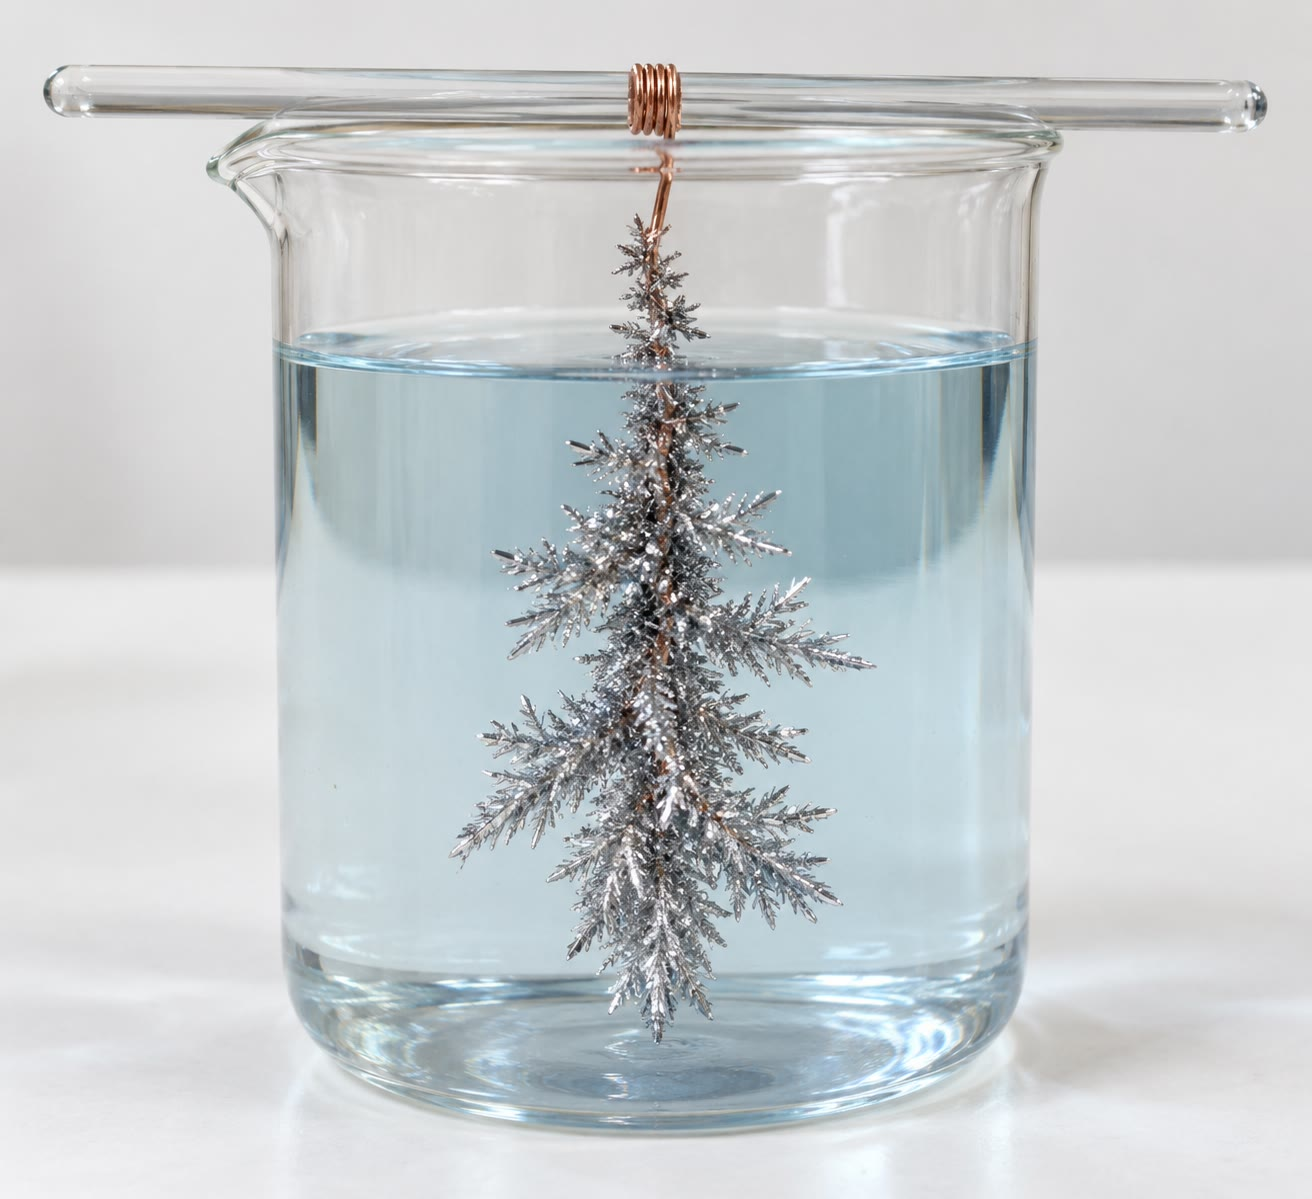
\includegraphics[width=0.5\linewidth]{images/book1/ai/g11-silver-tree.jpg}

{\small Kristal-kristal perak yang tumbuh pada kawat tembaga di dalam
larutan perak nitrat.}
\end{omfigure}

\section{Menyetarakan setengah reaksi}

Banyak pasangan penting yang mengandung oksigen dan ditulis untuk
\omterm{def:g9:acids-bases-ph:acidic}{larutan asam}, tempat \omterm{def:g9:ions:ion}{ion-ion} \ce{H+} berada. \omterm{def:g11:redox:couple}{Setengah reaksinya}
memerlukan \omterm{def:g7:atoms-and-molecules:molecule}{molekul} air dan \omterm{def:g9:ions:ion}{ion} \ce{H+} untuk disetarakan.

\begin{method}[Menyetarakan setengah reaksi dalam larutan asam]\label{met:g11:redox:balance}
Untuk menuliskan \omterm{def:g11:redox:couple}{setengah reaksi} pasangan Oks/Red dalam \omterm{def:g9:acids-bases-ph:acidic}{larutan asam}:
\begin{enumerate}
  \item tuliskan Oks di kiri dan Red di kanan, lalu setarakan \omterm{def:g7:atoms-and-molecules:atom}{atom} yang
        bukan O dan bukan H;
  \item setarakan \omterm{def:g7:atoms-and-molecules:atom}{atom} oksigen dengan \omterm{def:g7:atoms-and-molecules:molecule}{molekul} air \ce{H2O};
  \item setarakan \omterm{def:g7:atoms-and-molecules:atom}{atom} hidrogen dengan \omterm{def:g9:ions:ion}{ion} \ce{H+};
  \item setarakan muatan dengan \omterm{def:g9:inside-the-atom:nucleus}{elektron} \ce{e-}, di kiri;
  \item periksalah: banyaknya setiap \omterm{def:g7:atoms-and-molecules:atom}{atom} sama, dan muatan totalnya sama
        di kedua ruas.
\end{enumerate}
\end{method}

\begin{example}[Ion permanganat]\label{ex:g11:redox:permanganate}
Untuk pasangan \ce{MnO4^-}/\ce{Mn^{2+}} (ungu tua menjadi hampir tak
berwarna): mangan sudah setara; empat O di kiri memberikan
$\ce{4H2O}$ di kanan; kedelapan H-nya memberikan $\ce{8H+}$ di kiri;
muatan di kiri $-1 + 8 = +7$, di kanan $+2$, jadi lima \omterm{def:g9:inside-the-atom:nucleus}{elektron}
ditambahkan di kiri:
\[
  \ce{MnO4^-(aq) + 8H+(aq) + 5e- <=> Mn^{2+}(aq) + 4H2O(l)}.
\]
\end{example}

\begin{example}[Ion dikromat]\label{ex:g11:redox:dichromate}
Untuk \ce{Cr2O7^{2-}}/\ce{Cr^{3+}} (jingga menjadi hijau): dua kromium di
kanan; tujuh O memberikan \ce{7H2O}; empat belas H memberikan
\ce{14H+}; muatan $-2 + 14 = +12$ di kiri dibandingkan $2 \times 3 = +6$
di kanan, jadi enam \omterm{def:g9:inside-the-atom:nucleus}{elektron}:
\[
  \ce{Cr2O7^{2-}(aq) + 14H+(aq) + 6e- <=> 2Cr^{3+}(aq) + 7H2O(l)}.
\]
\end{example}

\begin{method}[Menuliskan persamaan redoks]\label{met:g11:redox:combine}
Untuk menuliskan \omterm{def:g8:balanced-equations:equation}{persamaan reaksi} antara \omterm{def:g11:redox:oxidant}{oksidator} Oks$_1$ dari satu
pasangan dan \omterm{def:g11:redox:oxidant}{reduktor} Red$_2$ dari pasangan lain:
\begin{enumerate}
  \item tuliskan kedua \omterm{def:g11:redox:couple}{setengah reaksi}, yang pertama dengan arah \omterm{def:g11:redox:oxidation}{reduksi}
        (Oks$_1 \to$ Red$_1$), yang kedua dengan arah \omterm{def:g11:redox:oxidation}{oksidasi}
        (Red$_2 \to$ Oks$_2$);
  \item kalikan keduanya dengan bilangan terkecil yang membuat
        \omterm{def:g9:inside-the-atom:nucleus}{elektronnya} sama;
  \item jumlahkan keduanya; \omterm{def:g9:inside-the-atom:nucleus}{elektron-elektronnya} saling meniadakan,
        begitu pula sebagian \ce{H+} dan \ce{H2O} yang muncul di kedua
        ruas;
  \item periksalah \omterm{def:g7:atoms-and-molecules:atom}{atom} dan muatannya sekali lagi.
\end{enumerate}
\end{method}

\begin{example}[Permanganat dan besi(II)]\label{ex:g11:redox:mno4-fe}
\omterm{def:g9:ions:ion}{Ion} permanganat mengoksidasi \omterm{def:g9:ions:ion}{ion-ion} \ce{Fe^{2+}} menjadi \ce{Fe^{3+}}:
\[
\begin{array}{l@{\qquad}l}
  \ce{MnO4^- + 8H+ + 5e- -> Mn^{2+} + 4H2O} & \times 1\\
  \ce{Fe^{2+} -> Fe^{3+} + e-} & \times 5\\
  \hline
  \ce{MnO4^- + 8H+ + 5Fe^{2+} -> Mn^{2+} + 5Fe^{3+} + 4H2O} &
\end{array}
\]
Muatan di kiri: $-1 + 8 + 10 = +17$; di kanan: $2 + 15 = +17$. Reaksi ini
dipakai pada bab berikutnya untuk mengukur jumlah besi(II).
\end{example}

\section{Oksidator dan reduktor di sekitar kita}

\begin{proposition}[Beberapa oksidator dan reduktor yang umum]\label{prop:g11:redox:common}
Spesies-spesies berikut dijumpai berulang kali di laboratorium dan dalam
kehidupan sehari-hari:
\begin{center}
\small
\begin{tabular}{lll}
\hline
spesies & peran & \omterm{def:g11:redox:couple}{setengah reaksi} pasangannya \\
\hline
oksigen \ce{O2} & \omterm{def:g11:redox:oxidant}{oksidator} & \ce{O2 + 4H+ + 4e- <=> 2H2O} \\
klorin \ce{Cl2} & \omterm{def:g11:redox:oxidant}{oksidator} & \ce{Cl2 + 2e- <=> 2Cl-} \\
hipoklorit \ce{ClO-} (pemutih) & \omterm{def:g11:redox:oxidant}{oksidator} & \ce{2ClO- + 4H+ + 2e- <=> Cl2 + 2H2O} \\
hidrogen peroksida \ce{H2O2} & \omterm{def:g11:redox:oxidant}{oksidator} & \ce{H2O2 + 2H+ + 2e- <=> 2H2O} \\
permanganat \ce{MnO4^-} & \omterm{def:g11:redox:oxidant}{oksidator} & \ce{MnO4^- + 8H+ + 5e- <=> Mn^{2+} + 4H2O} \\
\omterm{def:g9:periodic-table-first-look:metal}{logam} \ce{M} (\ce{Fe}, \ce{Zn}, \ce{Al}\dots) & \omterm{def:g11:redox:oxidant}{reduktor} & \ce{M^{n+} + $n$ e- <=> M} % ce-unbalanced-ok (generic)
\\
iodida \ce{I-} & \omterm{def:g11:redox:oxidant}{reduktor} & \ce{I2 + 2e- <=> 2I-} \\
tiosulfat \ce{S2O3^{2-}} & \omterm{def:g11:redox:oxidant}{reduktor} & \ce{S4O6^{2-} + 2e- <=> 2S2O3^{2-}} \\
asam askorbat \ce{C6H8O6} (vitamin C) & \omterm{def:g11:redox:oxidant}{reduktor} & \ce{C6H6O6 + 2H+ + 2e- <=> C6H8O6} \\
\hline
\end{tabular}
\end{center}
\end{proposition}

\begin{example}[Tembaga menjadi hijau]\label{ex:g11:redox:patina}
Atap dan patung tembaga, yang dibiarkan di \omterm{def:g4:air-a-mixture-of-gases:air}{udara} terbuka selama
puluhan tahun, perlahan berubah menjadi hijau pucat. Oksigen dari \omterm{def:g4:air-a-mixture-of-gases:air}{udara}
mengoksidasi tembaga menjadi \omterm{def:g9:ions:ion}{ion} \ce{Cu^{2+}}, yang bersama air dan
karbon dioksida membentuk kerak hijau yang tipis, yaitu patina. Tidak
seperti \omterm{def:g9:metals-acids-corrosion:corrosion}{karat} pada besi, patina melekat pada \omterm{def:g9:periodic-table-first-look:metal}{logam} dan melindunginya
dari serangan lebih lanjut.
\end{example}

\begin{omfigure}

\includegraphics[width=0.48\linewidth]{images/book1/ai/g11-green-roof.jpg}

{\small Atap tembaga setelah puluhan tahun di \omterm{def:g4:air-a-mixture-of-gases:air}{udara}: tembaga yang
teroksidasi membentuk patina hijau.}
\end{omfigure}

\begin{remark}[Antioksidan]\label{rem:g11:redox:antioxidant}
``Antioksidan'' yang ditambahkan pada makanan adalah \omterm{def:g11:redox:oxidant}{reduktor} yang
dioksidasi oleh oksigen \omterm{def:g4:air-a-mixture-of-gases:air}{udara} sebelum makanan itu teroksidasi. Vitamin C
(asam askorbat) adalah yang paling umum: apel yang dipotong lalu
diperciki air jeruk lemon jauh lebih lambat menjadi cokelat, karena
vitamin C dalam jeruk lemon dioksidasi lebih dulu.
\end{remark}

\section{Latihan}

\begin{exercise}[$\star$]\label{exo:g11:redox:1}
Definisikan \omterm{def:g11:redox:oxidant}{oksidator}, \omterm{def:g11:redox:oxidant}{reduktor}, \omterm{def:g11:redox:oxidation}{oksidasi}, dan \omterm{def:g11:redox:oxidation}{reduksi}.
\end{exercise}

\begin{exercise}[$\star$]\label{exo:g11:redox:2}
Untuk setiap pasangan, tuliskan \omterm{def:g11:redox:couple}{pasangan redoksnya} dalam bentuk Oks/Red:
\ce{Fe} dan \ce{Fe^{2+}}; \ce{Ag} dan \ce{Ag+}; \ce{I-} dan \ce{I2};
\ce{Fe^{2+}} dan \ce{Fe^{3+}}.
\end{exercise}

\begin{exercise}[$\star$]\label{exo:g11:redox:3}
Tuliskan \omterm{def:g11:redox:couple}{setengah reaksi} pasangan \ce{Ag+}/\ce{Ag},
\ce{Al^{3+}}/\ce{Al}, \ce{Fe^{3+}}/\ce{Fe^{2+}}, dan \ce{Cl2}/\ce{Cl-}.
\end{exercise}

\begin{exercise}[$\star$]\label{exo:g11:redox:4}
Apakah perubahan \ce{Fe -> Fe^{2+} + 2e-} sebuah \omterm{def:g11:redox:oxidation}{oksidasi} atau \omterm{def:g11:redox:oxidation}{reduksi}?
Apakah besi bertindak sebagai \omterm{def:g11:redox:oxidant}{oksidator} atau \omterm{def:g11:redox:oxidant}{reduktor}?
\end{exercise}

\begin{exercise}[$\star$]\label{exo:g11:redox:5}
Pada reaksi \ce{Zn + Cu^{2+} -> Zn^{2+} + Cu}, sebutkan spesies yang
dioksidasi, spesies yang direduksi, \omterm{def:g11:redox:oxidant}{oksidator}, dan \omterm{def:g11:redox:oxidant}{reduktornya}, lalu
berikan banyaknya \omterm{def:g9:inside-the-atom:nucleus}{elektron} yang berpindah untuk setiap \omterm{def:g7:atoms-and-molecules:atom}{atom} seng.
\end{exercise}

\begin{exercise}[$\star\star$]\label{exo:g11:redox:6}
Setarakan, dalam \omterm{def:g9:acids-bases-ph:acidic}{larutan asam}, \omterm{def:g11:redox:couple}{setengah reaksi} pasangan
\ce{H2O2}/\ce{H2O}, dengan mengikuti \cref{met:g11:redox:balance}
langkah demi langkah.
\end{exercise}

\begin{exercise}[$\star\star$]\label{exo:g11:redox:7}
Tuliskan \omterm{def:g8:balanced-equations:equation}{persamaan reaksi} antara iodin \ce{I2} dan \omterm{def:g9:ions:ion}{ion} tiosulfat
\ce{S2O3^{2-}}, yang menghasilkan \omterm{def:g9:ions:ion}{ion} iodida dan \omterm{def:g9:ions:ion}{ion} tetrationat
\ce{S4O6^{2-}}.
\end{exercise}

\begin{exercise}[$\star\star$]\label{exo:g11:redox:8}
Tuliskan \omterm{def:g8:balanced-equations:equation}{persamaan reaksi} pohon perak dari kedua \omterm{def:g11:redox:couple}{setengah reaksinya}, dan
jelaskan mengapa larutannya menjadi biru.
\end{exercise}

\begin{exercise}[$\star\star$]\label{exo:g11:redox:9}
Vitamin C, \ce{C6H8O6}, bereaksi dengan iodin \ce{I2}. Tuliskan
\omterm{def:g8:balanced-equations:equation}{persamaan reaksinya}, dan sebutkan spesies yang menjadi \omterm{def:g11:redox:oxidant}{reduktor}.
\end{exercise}

\begin{exercise}[$\star\star$]\label{exo:g11:redox:10}
Aluminium bereaksi dengan \omterm{def:g9:ions:ion}{ion} tembaga(II). Tuliskan persamaannya, dan
jelaskan mengapa setengah-setengah reaksinya harus dikalikan dengan 2
dan dengan 3.
\end{exercise}

\begin{exercise}[$\star\star$]\label{exo:g11:redox:11}
Hidrogen peroksida mengoksidasi \omterm{def:g9:ions:ion}{ion} besi(II) menjadi \omterm{def:g9:ions:ion}{ion} besi(III) dalam
\omterm{def:g9:acids-bases-ph:acidic}{larutan asam}. Tuliskan persamaannya.
\end{exercise}

\begin{exercise}[$\star\star\star$]\label{exo:g11:redox:12}
Sekeping seng kehilangan \qty{1.30}{g} di dalam larutan yang mengandung
\omterm{def:g9:ions:ion}{ion} tembaga(II) berlebih. Berapa massa tembaga yang mengendap? Pakailah
$M(\ce{Zn}) = \qty{65.4}{g/mol}$ dan $M(\ce{Cu}) = \qty{63.5}{g/mol}$.
\end{exercise}

\begin{exercise}[$\star\star\star$]\label{exo:g11:redox:13}
Tuliskan persamaan \omterm{def:g11:redox:oxidation}{oksidasi} \omterm{def:g9:ions:ion}{ion} besi(II) oleh \omterm{def:g9:ions:ion}{ion} dikromat dalam \omterm{def:g9:acids-bases-ph:acidic}{larutan
asam}. Berapa jumlah \ce{Fe^{2+}} yang dioksidasi oleh \qty{0.010}{mol}
\omterm{def:g9:ions:ion}{ion} dikromat?
\end{exercise}

\begin{exercise}[$\star\star\star$]\label{exo:g11:redox:14}
Pemutih mengandung \omterm{def:g9:ions:ion}{ion} hipoklorit \ce{ClO-} dan \omterm{def:g9:ions:ion}{ion} klorida \ce{Cl-}.
Dengan pasangan \ce{ClO-}/\ce{Cl2} dan \ce{Cl2}/\ce{Cl-}, tuliskan
\omterm{def:g8:balanced-equations:equation}{persamaan reaksi} yang terjadi ketika pemutih bertemu asam, dan jelaskan
mengapa label pemutih maupun label produk pembersih kerak yang asam
sama-sama memperingatkan agar keduanya tidak pernah \omterm{def:g2:mixing-and-dissolving:mix}{dicampur}.
\end{exercise}

\begin{exercise}[$\star\star\star$]\label{exo:g11:redox:15}
Pada gambar permukaan seng, \omterm{def:g9:inside-the-atom:nucleus}{elektron-elektron} bergerak melalui \omterm{def:g9:periodic-table-first-look:metal}{logam},
bukan melalui larutan. Dengan \cref{prop:g11:redox:no-free-electrons},
jelaskan mengapa tembaga mengendap pada keping seng itu sendiri dan
bukan di tempat lain di dalam gelas kimia.
\end{exercise}

\section{Soal: Tes Napas}

\begin{problem}[{Soal akhir pekan --- kimia tabung tes alkohol napas: dua
pasangan, perubahan warna jingga ke hijau, massa etanol yang dapat
dideteksi sebuah tabung, dan sel bahan bakar yang menggantikannya}]
\label{pb:g11:redox:1}
% ledger: ghs:K2Cr2O7, breath:ratio; molar masses from tools/molar_mass.py
% (0.1-rounded weights): K2Cr2O7 294.2, C2H6O 46.0 g/mol
Tes \omterm{def:g11:functional-groups:alcohol}{alkohol} napas yang pertama memakai tabung kaca berisi butiran silika
yang dilapisi kalium dikromat berwarna jingga, \ce{K2Cr2O7}, dalam
suasana asam. Etanol, \ce{CH3CH2OH}, dalam napas yang diembuskan melalui
tabung itu mereduksi \omterm{def:g9:ions:ion}{ion-ion} dikromat menjadi \omterm{def:g9:ions:ion}{ion} \ce{Cr^{3+}} yang hijau
dan dioksidasi menjadi asam etanoat, \ce{CH3COOH}; panjang daerah hijau
itu mengukur etanolnya. Anggaplah sebuah tabung mengandung
\qty{2.0}{mg} kalium dikromat. Pakailah
$M(\ce{K}) = 39.1$, $M(\ce{Cr}) = 52.0$, $M(\ce{O}) = 16.0$,
$M(\ce{C}) = 12.0$, $M(\ce{H}) = \qty{1.0}{g/mol}$, $N_A =
\qty{6.02e23}{mol^{-1}}$, dan $e = \qty{1.60e-19}{C}$.

\medskip
\noindent\textbf{Bagian I --- Dua pasangan.}
\begin{enumerate}
  \item Sebutkan kedua \omterm{def:g11:redox:couple}{pasangan redoks} yang terlibat, \omterm{def:g11:redox:oxidant}{oksidator} di depan.
  \item Apakah etanol dioksidasi atau direduksi? Apakah etanol
        \omterm{def:g11:redox:oxidant}{oksidator} atau \omterm{def:g11:redox:oxidant}{reduktor}?
  \item Tuliskan \omterm{def:g11:redox:couple}{setengah reaksi} pasangan \ce{Cr2O7^{2-}}/\ce{Cr^{3+}}
        dalam \omterm{def:g9:acids-bases-ph:acidic}{larutan asam}.
  \item Tuliskan \omterm{def:g11:redox:couple}{setengah reaksi} pasangan \ce{CH3COOH}/\ce{CH3CH2OH}
        dalam \omterm{def:g9:acids-bases-ph:acidic}{larutan asam}.
  \item Simpulkan \omterm{def:g8:balanced-equations:equation}{persamaan reaksi} di dalam tabung.
\end{enumerate}

\medskip
\noindent\textbf{Bagian II --- Yang dapat diukur satu tabung.}
\begin{enumerate}[resume]
  \item Jelaskan perubahan warna butiran-butiran itu.
  \item Hitung \omterm{def:g10:the-mole:molar-mass}{massa molar} kalium dikromat.
  \item Hitung jumlah \omterm{def:g9:ions:ion}{ion} dikromat di dalam tabung.
  \item Berapa jumlah etanol yang diperlukan untuk membuat seluruh tabung
        menjadi hijau?
  \item Simpulkan massa etanol terbesar yang dapat diukur satu tabung.
\end{enumerate}

\medskip
\noindent\textbf{Bagian III --- Dari napas ke darah.}
Seseorang mengembuskan \qty{1.0}{L} napas melalui tabung itu; daerah
hijaunya bertambah panjang sebanding dengan massa etanol yang
mencapainya.
\begin{enumerate}[resume]
  \item Napas itu mengandung \qty{0.25}{mg} etanol per liter. Berapa
        bagian dikromat yang terpakai?
  \item Tabung itu panjangnya \qty{10}{cm}. Berapa panjang daerah
        hijaunya?
  \item Alat analisis napas menganggap bahwa \qty{2100}{L} napas
        membawa etanol sebanyak \qty{1}{L} darah. Perkirakan massa etanol
        per liter darah, dalam gram.
  \item Mengapa daerah hijau itu mulai dari lubang masuk tabung dan
        bertambah ke arah lubang keluar, alih-alih seluruh tabung menjadi
        sedikit hijau?
  \item Mengapa sebuah tabung hanya dapat dipakai sekali?
\end{enumerate}

\medskip
\noindent\textbf{Bagian IV --- Sel \omterm{def:g4:what-a-fire-needs:fuel}{bahan bakar}.}
Kalium dikromat memuat piktogram
\ghs[0.6cm]{GHS03}\,\ghs[0.6cm]{GHS05}\,\ghs[0.6cm]{GHS06}\,\ghs[0.6cm]{GHS07}\,\ghs[0.6cm]{GHS08}\,\ghs[0.6cm]{GHS09}.
Alat-alat modern memakai sel \omterm{def:g4:what-a-fire-needs:fuel}{bahan bakar} sebagai gantinya, tempat etanol
dalam napas dioksidasi oleh oksigen pada sebuah elektrode, dan \omterm{def:g9:inside-the-atom:nucleus}{elektron}
yang dilepaskan mengalir melalui kawat.
\begin{enumerate}[resume]
  \item Berikan dua alasan, yang dibaca dari piktogram-piktogram itu,
        mengapa tabung dikromat ditinggalkan.
  \item Tuliskan persamaan \omterm{def:g11:redox:oxidation}{oksidasi} etanol oleh oksigen, dengan memakai
        pasangan \ce{O2}/\ce{H2O}.
  \item Berapa \omterm{def:g9:inside-the-atom:nucleus}{elektron} yang dilepaskan satu \omterm{def:g7:atoms-and-molecules:molecule}{molekul} etanol ketika
        dioksidasi menjadi asam etanoat?
  \item Untuk \qty{0.25}{mg} etanol, hitung jumlah etanolnya, lalu
        banyaknya \omterm{def:g9:inside-the-atom:nucleus}{elektron} yang dilepaskan.
  \item Simpulkan muatan listrik yang mengalir melalui sel \omterm{def:g4:what-a-fire-needs:fuel}{bahan bakar}
        itu. Mengapa muatan ini merupakan ukuran yang baik untuk etanol
        dalam napas?
\end{enumerate}
\end{problem}
